% Options for packages loaded elsewhere
\PassOptionsToPackage{unicode}{hyperref}
\PassOptionsToPackage{hyphens}{url}
%
\documentclass[
]{article}
\usepackage{amsmath,amssymb}
\usepackage{lmodern}
\usepackage{iftex}
\ifPDFTeX
  \usepackage[T1]{fontenc}
  \usepackage[utf8]{inputenc}
  \usepackage{textcomp} % provide euro and other symbols
\else % if luatex or xetex
  \usepackage{unicode-math}
  \defaultfontfeatures{Scale=MatchLowercase}
  \defaultfontfeatures[\rmfamily]{Ligatures=TeX,Scale=1}
\fi
% Use upquote if available, for straight quotes in verbatim environments
\IfFileExists{upquote.sty}{\usepackage{upquote}}{}
\IfFileExists{microtype.sty}{% use microtype if available
  \usepackage[]{microtype}
  \UseMicrotypeSet[protrusion]{basicmath} % disable protrusion for tt fonts
}{}
\makeatletter
\@ifundefined{KOMAClassName}{% if non-KOMA class
  \IfFileExists{parskip.sty}{%
    \usepackage{parskip}
  }{% else
    \setlength{\parindent}{0pt}
    \setlength{\parskip}{6pt plus 2pt minus 1pt}}
}{% if KOMA class
  \KOMAoptions{parskip=half}}
\makeatother
\usepackage{xcolor}
\IfFileExists{xurl.sty}{\usepackage{xurl}}{} % add URL line breaks if available
\IfFileExists{bookmark.sty}{\usepackage{bookmark}}{\usepackage{hyperref}}
\hypersetup{
  hidelinks,
  pdfcreator={LaTeX via pandoc}}
\urlstyle{same} % disable monospaced font for URLs
\usepackage{longtable,booktabs,array}
\usepackage{calc} % for calculating minipage widths
% Correct order of tables after \paragraph or \subparagraph
\usepackage{etoolbox}
\makeatletter
\patchcmd\longtable{\par}{\if@noskipsec\mbox{}\fi\par}{}{}
\makeatother
% Allow footnotes in longtable head/foot
\IfFileExists{footnotehyper.sty}{\usepackage{footnotehyper}}{\usepackage{footnote}}
\makesavenoteenv{longtable}
\usepackage{graphicx}
\makeatletter
\def\maxwidth{\ifdim\Gin@nat@width>\linewidth\linewidth\else\Gin@nat@width\fi}
\def\maxheight{\ifdim\Gin@nat@height>\textheight\textheight\else\Gin@nat@height\fi}
\makeatother
% Scale images if necessary, so that they will not overflow the page
% margins by default, and it is still possible to overwrite the defaults
% using explicit options in \includegraphics[width, height, ...]{}
\setkeys{Gin}{width=\maxwidth,height=\maxheight,keepaspectratio}
% Set default figure placement to htbp
\makeatletter
\def\fps@figure{htbp}
\makeatother
\setlength{\emergencystretch}{3em} % prevent overfull lines
\providecommand{\tightlist}{%
  \setlength{\itemsep}{0pt}\setlength{\parskip}{0pt}}
\setcounter{secnumdepth}{5}
\usepackage[utf8]{inputenc}
\usepackage{fontspec}
%\setmainfont{Calibri}
\renewcommand{\baselinestretch}{1.2}
\usepackage{amsmath}
\usepackage{graphicx}
\usepackage{enumitem}
\graphicspath{{images/}}
\usepackage[labelformat=simple]{caption}
\usepackage[figurename=Figure]{caption}
\usepackage[a4paper,width=150mm,top=25mm,bottom=25mm]{geometry}
\usepackage{tikz}
%\usepackage[colorlinks]{hyperref}
\hypersetup{linkcolor=black}
\usepackage[nameinlink,noabbrev]{cleveref}
\usepackage{pgfplots}
\usepackage{algorithm}
\usepackage{algpseudocode}
\pagestyle{plain}
\bibliographystyle{unsrt}
\hypersetup{%
  citecolor=black
}
\usepackage{amssymb}
\newcommand{\comment}[1]{}
\pgfplotsset{compat=1.17} 
\usepackage{float}
\usepackage{booktabs}
\usepackage{longtable}
\usepackage{array}
\usepackage{multirow}
\usepackage{wrapfig}
\usepackage{float}
\usepackage{colortbl}
\usepackage{pdflscape}
\usepackage{tabu}
\usepackage{threeparttable}
\usepackage{threeparttablex}
\usepackage[normalem]{ulem}
\usepackage{makecell}
\usepackage{xcolor}
\ifLuaTeX
  \usepackage{selnolig}  % disable illegal ligatures
\fi

\author{}
\date{\vspace{-2.5em}}

\begin{document}


\begin{titlepage}
\newcommand{\HRule}{\rule{\linewidth}{0.5mm}} % Defines a new command for the horizontal lines, change thickness here

\thispagestyle{empty}

\vfill
\begin{center}

\includegraphics[width=200pt,  keepaspectratio]{logo.png}
\end{center}

\vspace*{45mm}
\begin{center}
{\LARGE \textmd{}}\\\vspace*{3mm}
\Huge\HRule\\[0.4cm]{\textbf{Statistical Analysis of Reliability and Survival Data:\\
Rotterdam Dataset}}
\HRule\\[100pt] %20pt

\large \textbf{Authors} \\
\large \textmd{
    Aksoy, Barış r0869901 \\
   Heller, Jack r0862809 \\
    Zdravković, Aleksandra r0869484
} \\\vspace*{5mm}

\vfill

\centerline{\large \textmd{Leuven. May, 2022}}
\end{center}

\end{titlepage}

\section{Exploratory Data Analysis}

These data sets are used in the paper by Royston and Altman that is
referenced below. The Rotterdam data is used to create a fitted model,
and the GBSG data for validation of the model. The paper gives
references for the data source.

There are 43 subjects who have died without recurrence, but whose death
time is greater than the censoring time for recurrence. A common way
that this happens is that a death date is updated in the health record
sometime after the research study ended, and said value is then picked
up when a study data set is created. But it raises serious questions
about censoring. For instance subject 40 is censored for recurrence at
4.2 years and died at 6.6 years; when creating the endpoint of
recurrence free survival (earlier of recurrence or death), treating them
as a death at 6.6 years implicitly assumes that they were recurrence
free just before death. For this to be true we would have to assume that
if they had progressed in the 2.4 year interval before death (while off
study), that this information would also have been noted in their
general medical record, and would also be captured in the study data
set. However, that may be unlikely. Death information is often in a
centralized location in electronic health records, easily accessed by a
programmer and merged with the study data, while recurrence may require
manual review. How best to address this is an open issue.

\begin{table}[!h]

\caption{\label{tab:data-desc}Data description}
\centering
\begin{tabular}[t]{ll}
\toprule
\cellcolor{gray!6}{pid} & \cellcolor{gray!6}{Patient identifier}\\
year & Year of surgery\\
\cellcolor{gray!6}{age} & \cellcolor{gray!6}{Age at surgery}\\
meno & Menopausal status (0 = premenopausal, 1 = postmenopausal)\\
\cellcolor{gray!6}{size} & \cellcolor{gray!6}{Tumor size, a factor with levels <= 20, 20-25, > 50}\\
\addlinespace
grade & Differentiation grade\\
\cellcolor{gray!6}{nodes} & \cellcolor{gray!6}{Number of positive lymph nodes}\\
pgr & Progesterone receptors (fmol/l)\\
\cellcolor{gray!6}{er} & \cellcolor{gray!6}{Estrogen receptors (fmol/l)}\\
hormon & Hormonal treatment (0=no, 1=yes)\\
\addlinespace
\cellcolor{gray!6}{chemo} & \cellcolor{gray!6}{Chemotherapy}\\
rtime & Days to relapse or last follow-up\\
\cellcolor{gray!6}{recur} & \cellcolor{gray!6}{0 = no relapse, 1 = relapse}\\
dtime & Days to death or last follow-up\\
\cellcolor{gray!6}{death} & \cellcolor{gray!6}{0 = alive, 1 = dead}\\
\bottomrule
\end{tabular}
\end{table}

Table \ref{tab:data-desc} explains the covariates in the Rotterdam
dataset.

\subsection{Categorical Variables}

When we investigate the categorical variables, we see that some have a larger difference between time until death than others. When we first investigate menopause, we see that menopausal patients are very similar in their death time. A very similar pattern is observed for chemotherapy but the patients that did not die had a slightly higher time before leaving the study. While size, having three levels, needs to be interpreted slightly differently. With patients that died, the larger cancer cells certainly caused it to happen sooner. This makes intuitive sense that more severe cancer would have more long term health risks. Among patients that do not die, only the extremely large cancer patients had a much lower recurrence time. While small and medium patients had a very similar response. Grade had a very similar response among all patients with higher grade patients living slightly shorter lives. Patients given hormonal therapy seem to have a smaller tail among patients that died; meaning those who relapse are more likely to do it soon after treatment. Surviving patients that had hormonal therapy also appear to be censored more quickly than those who do not receive the treatment.

\includegraphics[width=0.5\linewidth,]{project_files/figure-latex/boxPlots-1} \includegraphics[width=0.5\linewidth,]{project_files/figure-latex/boxPlots-2} \includegraphics[width=0.5\linewidth,]{project_files/figure-latex/boxPlots-3} \includegraphics[width=0.5\linewidth,]{project_files/figure-latex/boxPlots-4} \includegraphics[width=0.5\linewidth,]{project_files/figure-latex/boxPlots-5}

\subsection{Continuous Variables}

Among continuous variables, we first investigated age. We plotted a both the lowess curve and the linear model to see if they match. If so, they most likely have data with a limited skew and do not require transformation for modeling. We first evaluated age and there was not a difference between the linear and lowess curves. Next, we investigated the relationship between er and death time. Here we see a large deviation which was corrected for again with a log transform. Finally, we evaluated pgr and it had a good fit overall.

\includegraphics[width=0.5\linewidth,]{project_files/figure-latex/scatterPlots-1} \includegraphics[width=0.5\linewidth,]{project_files/figure-latex/scatterPlots-2} \includegraphics[width=0.5\linewidth,]{project_files/figure-latex/scatterPlots-3} \includegraphics[width=0.5\linewidth,]{project_files/figure-latex/scatterPlots-4}

\section{Further Analysis}

Now the focus will be on the response variable, the censoring indicator,
and the categorical variable.

\subsection{Survival Distrubution by Levels of \textit{Size}, \textit{Meno}, \textit{Hormon}, and \textit{Chemo}}

For each of the levels of the categorical variables, we will compute the survival distribution and interpret the results.

\subsubsection{Size}

\begin{center}\includegraphics[width=0.85\linewidth,]{project_files/figure-latex/unnamed-chunk-3-1} \end{center}

The horizontal axis represents time in days, and the vertical axis shows
the probability of surviving, or the proportion of people surviving. The
lines represent survival curves of the three groups. A vertical drop in
the curves indicates an event. The vertical tick mark on the curves
means that a patient was censored at this time.

\begin{table}[!h]

\caption{\label{tab:median-size}Summary of the model.}
\centering
\fontsize{8}{10}\selectfont
\begin{tabular}[t]{lrrrrrrrrr}
\toprule
  & records & n.max & n.start & events & rmean & se(rmean) & median & 0.95LCL & 0.95UCL\\
\midrule
\cellcolor{gray!6}{Size ($\leq$20)} & \cellcolor{gray!6}{1387} & \cellcolor{gray!6}{1387} & \cellcolor{gray!6}{1387} & \cellcolor{gray!6}{414} & \cellcolor{gray!6}{4721.199} & \cellcolor{gray!6}{119.40159} & \cellcolor{gray!6}{5653} & \cellcolor{gray!6}{4983} & \cellcolor{gray!6}{}\\
Size (20$-$50) & 1291 & 1291 & 1291 & 646 & 3807.025 & 95.52799 & 3386 & 3084 & 3690\\
\cellcolor{gray!6}{Size ($>$50)} & \cellcolor{gray!6}{304} & \cellcolor{gray!6}{304} & \cellcolor{gray!6}{304} & \cellcolor{gray!6}{212} & \cellcolor{gray!6}{2537.178} & \cellcolor{gray!6}{148.10071} & \cellcolor{gray!6}{1909} & \cellcolor{gray!6}{1566} & \cellcolor{gray!6}{2141}\\
\bottomrule
\end{tabular}
\end{table}

At time zero, the survival probability is 1.0 (or 100\% of the participants are alive). At time 2250, the probability of survival is approximately 0.625 for size\textgreater=50, and 0.85 for size\textless50.

From Table \ref{tab:median-size} can be seen that the median survival for Size \geq 50 is 5653, for Size 20-50 is 3386, and for Size \textgreater{} 50 is 1909. This suggests worse survival for patients with tumor of larger size. However, to evaluate whether this difference is statistically significant requires a formal statistical test, a subject that is discussed in the next sections.

\subsubsection{Menopause}

\begin{center}\includegraphics[width=0.85\linewidth,]{project_files/figure-latex/unnamed-chunk-5-1} \end{center}

\begin{table}[!h]

\caption{\label{tab:median-meno}Median survival times for each group.}
\centering
\fontsize{8}{10}\selectfont
\begin{tabular}[t]{lrrrrrrrrr}
\toprule
  & records & n.max & n.start & events & rmean & se(rmean) & median & 0.95LCL & 0.95UCL\\
\midrule
\cellcolor{gray!6}{Meno = 0} & \cellcolor{gray!6}{1312} & \cellcolor{gray!6}{1312} & \cellcolor{gray!6}{1312} & \cellcolor{gray!6}{468} & \cellcolor{gray!6}{4622.427} & \cellcolor{gray!6}{108.80722} & \cellcolor{gray!6}{5653} & \cellcolor{gray!6}{4983} & \cellcolor{gray!6}{}\\
Meno = 1 & 1670 & 1670 & 1670 & 804 & 3672.887 & 92.46545 & 3632 & 3368 & 3813\\
\bottomrule
\end{tabular}
\end{table}

At time zero, the survival probability is 1.0 (or 100\% of the
participants are alive). At time 2200, the probability of survival is
approximately 0.75 for non-menopausal patients, and 0.825 for
menopausal patients.

From Table \ref{tab:median-meno} can be seen that the median survival is 5653 for non-menopausal patients, and 3632 for menopausal, suggesting worse survival for patients that have gone through
menopause.

\subsubsection{Hormonal Treatment}

\begin{center}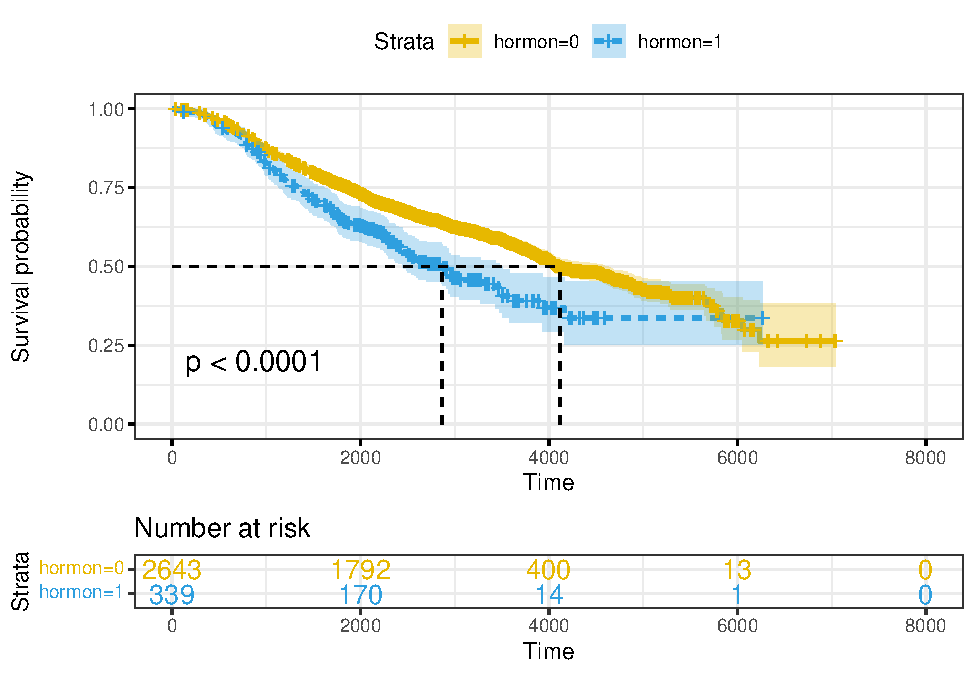
\includegraphics[width=0.85\linewidth,]{project_files/figure-latex/unnamed-chunk-7-1} \end{center}

\begin{table}[!h]

\caption{\label{tab:median-hormon}Median survival times for each group.}
\centering
\fontsize{8}{10}\selectfont
\begin{tabular}[t]{l|r|r|r|r|r|r|r|r|r}
\hline
  & records & n.max & n.start & events & rmean & se(rmean) & median & 0.95LCL & 0.95UCL\\
\hline
\cellcolor{gray!6}{hormon=0} & \cellcolor{gray!6}{2643} & \cellcolor{gray!6}{2643} & \cellcolor{gray!6}{2643} & \cellcolor{gray!6}{1113} & \cellcolor{gray!6}{4159.588} & \cellcolor{gray!6}{76.57099} & \cellcolor{gray!6}{4118} & \cellcolor{gray!6}{3988} & \cellcolor{gray!6}{4614}\\
\hline
hormon=1 & 339 & 339 & 339 & 159 & 3659.665 & 203.38456 & 2866 & 2450 & 3472\\
\hline
\end{tabular}
\end{table}

At time zero, the survival probability is 1.0 (or 100\% of the
participants are alive). At time 2200, the probability of survival is
approximately 0.75 for premenopausal patients, and 0.825 for
postmenopausal patients.

From Table \ref{tab:median-hormon} can be seen that the median survival is 4118 for patients that went through hormonal therapy, and 2866 for those who did not, suggesting slightly worse survival for patients that have gone through the hormonal therapy. However, to evaluate whether this difference is statistically significant requires a formal statistical test, a subject that is discussed in the next sections.

\subsubsection{Chemotherapy}

\begin{center}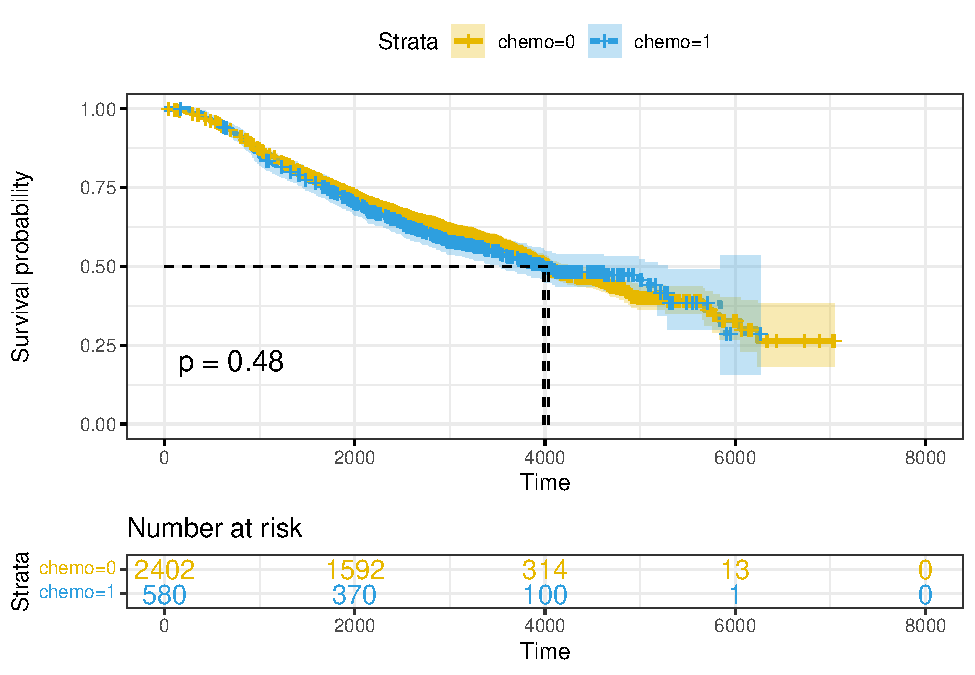
\includegraphics[width=0.85\linewidth,]{project_files/figure-latex/unnamed-chunk-9-1} \end{center}

\begin{table}[!h]

\caption{\label{tab:median-chemo}Median survival times for each group.}
\centering
\fontsize{8}{10}\selectfont
\begin{tabular}[t]{l|r|r|r|r|r|r|r|r|r}
\hline
  & records & n.max & n.start & events & rmean & se(rmean) & median & 0.95LCL & 0.95UCL\\
\hline
\cellcolor{gray!6}{chemo=0} & \cellcolor{gray!6}{2402} & \cellcolor{gray!6}{2402} & \cellcolor{gray!6}{2402} & \cellcolor{gray!6}{1014} & \cellcolor{gray!6}{4103.663} & \cellcolor{gray!6}{80.06765} & \cellcolor{gray!6}{4033} & \cellcolor{gray!6}{3885} & \cellcolor{gray!6}{4239}\\
\hline
chemo=1 & 580 & 580 & 580 & 258 & 4080.311 & 162.59049 & 3990 & 3522 & 5291\\
\hline
\end{tabular}
\end{table}

At time zero, the survival probability is 1.0 (or 100\% of the
participants are alive). At time 2200, the probability of survival is
approximately 0.75 for premenopausal patients, and 0.825 for
postmenopausal patients.

From Table \ref{tab:median-chemo} can be seen that the median survival is 4118 for patients that went through hormonal therapy, and 2866 for those who did not, suggesting slightly better survival for patients that have gone through chemotherapy. However, to evaluate whether this difference is statistically significant requires a formal statistical test, a subject that is discussed in the next sections.

\subsection{Confidence Intervals and Estimators by Levels of \textit{Size}, \textit{Meno}, \textit{Hormon}, and \textit{Chemo}}

For each level we will obtain an appropriate estimator and confidence interval for the 3 quartiles of the survival curves and interpret the results.

\begin{table}[!h]

\caption{\label{tab:quantiles-chemo}Estimates and confidence intervals for 3 quartiles for each level of covariates $\textit{size, chemo, meno, hormon}$.}
\centering
\fontsize{10}{12}\selectfont
\begin{tabular}[t]{lrrrrrllll}
\toprule
  & $\hat{q_1}$ & 5\% & 95\% & $\hat{q_2}$ & 5\% & 95\% & $\hat{q_3}$ & 5\% & 95\%\\
\midrule
\cellcolor{gray!6}{Size ($\leq$20)} & \cellcolor{gray!6}{2880} & \cellcolor{gray!6}{2590} & \cellcolor{gray!6}{3315} & \cellcolor{gray!6}{5653} & \cellcolor{gray!6}{4983} & \cellcolor{gray!6}{$\textit{NA}$} & \cellcolor{gray!6}{$\textit{NA}$} & \cellcolor{gray!6}{6051} & \cellcolor{gray!6}{$\textit{NA}$}\\
Size (20$-$50) & 1476 & 1361 & 1623 & 3386 & 3084 & 3690 & $\textit{NA}$ & 5830 & $\textit{NA}$\\
\cellcolor{gray!6}{Size ($>$50)} & \cellcolor{gray!6}{890} & \cellcolor{gray!6}{809} & \cellcolor{gray!6}{999} & \cellcolor{gray!6}{1909} & \cellcolor{gray!6}{1566} & \cellcolor{gray!6}{2141} & \cellcolor{gray!6}{3714} & \cellcolor{gray!6}{3240} & \cellcolor{gray!6}{4309}\\
Chemo = 0 & 1812 & 1677 & 1957 & 4033 & 3885 & 4239 & $\textit{NA}$ & 6051 & $\textit{NA}$\\
\cellcolor{gray!6}{Chemo = 1} & \cellcolor{gray!6}{1699} & \cellcolor{gray!6}{1455} & \cellcolor{gray!6}{1954} & \cellcolor{gray!6}{3990} & \cellcolor{gray!6}{3522} & \cellcolor{gray!6}{5291} & \cellcolor{gray!6}{$\textit{NA}$} & \cellcolor{gray!6}{5845} & \cellcolor{gray!6}{$\textit{NA}$}\\
\addlinespace
Meno = 0 & 2115 & 1944 & 2371 & 5653 & 4983 & $\textit{NA}$ & $\textit{NA}$ & $\textit{NA}$ & $\textit{NA}$\\
\cellcolor{gray!6}{Meno = 1} & \cellcolor{gray!6}{1571} & \cellcolor{gray!6}{1424} & \cellcolor{gray!6}{1723} & \cellcolor{gray!6}{3632} & \cellcolor{gray!6}{3368} & \cellcolor{gray!6}{3813} & \cellcolor{gray!6}{5762} & \cellcolor{gray!6}{5266} & \cellcolor{gray!6}{$\textit{NA}$}\\
Hormon = 0 & 1882 & 1742 & 1994 & 4118 & 3988 & 4614 & $\textit{NA}$ & 6051 & $\textit{NA}$\\
\cellcolor{gray!6}{Hormon = 1} & \cellcolor{gray!6}{1361} & \cellcolor{gray!6}{1140} & \cellcolor{gray!6}{1618} & \cellcolor{gray!6}{2866} & \cellcolor{gray!6}{2450} & \cellcolor{gray!6}{3472} & \cellcolor{gray!6}{$\textit{NA}$} & \cellcolor{gray!6}{$\textit{NA}$} & \cellcolor{gray!6}{$\textit{NA}$}\\
\bottomrule
\end{tabular}
\end{table}

We first evaluate size and see similar results to what was observed in the EDA barcharts. We see that at the 25th percentile, size \textgreater50 has a very significant difference from the other two groups. With this being significantly smaller, their dtime is significantly smaller. This intuitively makes sense that a person who has larger cancer would have a worse life expectancy. However, this phenomenon has faded by the 50th percentile and persists through the 75th. This means that if a person survives the initial hurdle after surgery, they are not expected to be significantly different from the rest of the population.

When we investigate the effect of menopause on survival, we see that generally people that are menopausal have lower survival times. This is supported by that at the 25th, 50th, and 75th percentiles, there is no overlap in the quantiles' confidence intervals. This means that at all stages, a menopausal person would have a shorter life. However, this could be due to other covariates such as the fact that all menopausal people are women or that they tend to be older.

We next evaluate the effect of hormonal treatment. We see here that those who received hormonal treatment generally have a lower survival time. We also see that there is no overlap between the confidence intervals indicating that not only did they have a large difference, but it sustained itself throughout the entire distribution of patients.

Finally, we evaluate the effect of chemotherapy. Here we see that generally chemotherapy patients live longer. However, this only becomes significant at the 75th percentile. This means that generally patients that receive chemotherapy are not significantly affected until they live for a long time.

\subsection{Test of Differences Between the Survival Curves}

\begin{table}[!h]

\caption{\label{tab:stratify}Stratified log-rank test for differences in menopause.}
\centering
\fontsize{10}{12}\selectfont
\begin{tabular}[t]{lrrr}
\toprule
  & $\chi^2$ & df & p-value\\
\midrule
\cellcolor{gray!6}{Stratified by Chemo} & \cellcolor{gray!6}{69.59} & \cellcolor{gray!6}{1} & \cellcolor{gray!6}{0}\\
Stratified by Size & 42.53 & 1 & 0\\
\cellcolor{gray!6}{Stratified by Hormon} & \cellcolor{gray!6}{44.06} & \cellcolor{gray!6}{1} & \cellcolor{gray!6}{0}\\
\bottomrule
\end{tabular}
\end{table}

\begin{figure}[H]

{\centering \includegraphics[width=0.85\linewidth,]{project_files/figure-latex/stratify-size-plot-1} 

}

\caption{Independent variable meno stratified by size of the tumor.}\label{fig:stratify-size-plot}
\end{figure}

In this setting we chose to use the log-rank test. This is because we do not want to weight any observations more heavily than others. Thus, we set \(W(Y(j)) = 1\). The log-rank test is the most powerful so it is the best choice. However, this test is only the most powerful when the hazard rates are proportional to each other within populations. For this reason, we stratify the model to identify its impacts and make sure no assumptions are violated.

What we see when we perform this stratification is a very large difference between someone without menopause and small cancer cells and someone who is menopausal and has very large cancer cells. We also see that stratifying on age has the best fit.

\section{Modeling}

\subsection {Semiparametric Proportional Hazards Model}

For semiparametric proportional hazards model, we proceed as follows:

The variable \textit{size} is a categorical variable with 3 levels. We recode the levels Size (\(20-50\)) and Size (\(>50\)) as binary variables, and take the level Size (\(\leq20\)) as reference level.
We then estimate the full model, only excluding variables \textit{rtime} and \textit{recur}, since they are not the chosen event of interest.

\begin{table}[!h]

\caption{\label{tab:AIC-table}AIC values for models selected by stepwise AIC procedure, and backward selection procedure. }
\centering
\fontsize{10}{12}\selectfont
\begin{tabular}[t]{lrr}
\toprule
  & Stepwise AIC & Backward Selection\\
\midrule
\cellcolor{gray!6}{AIC} & \cellcolor{gray!6}{18543.63} & \cellcolor{gray!6}{18546.82}\\
\bottomrule
\end{tabular}
\end{table}

For model selection with all covariates, we first fit a full model to apply backward selection procedure. By excluding the covariate with the largest p-value in each iteration, we ended up with the model where significant covariates are \textit{size, age, grade, nodes, pgr, meno, hormon}.

Next, we run stepwise AIC selection in both directions. This resulted with the model where significant covariates are \textit{size, age, grade, nodes, pgr}.

To decide which procedure should be used to choose the model, we approach from 2 different points. From a logical point of view, the model including hormonal treatment is reasonable since it might have a direct influence on survival time. If we compare AIC of both models, from Table \ref{tab:AIC-table} we see that there is no huge difference (\ensuremath{1.8544\times 10^{4}} and \ensuremath{1.8547\times 10^{4}}, respectively). So we decide to go with the model selected based on p-value since it includes hormon in exchange of acceptable increase in AIC.

\begin{table}[!h]

\caption{\label{tab:relative-risks-tbl}Relative risks and CI for each covariate}
\centering
\fontsize{10}{12}\selectfont
\begin{tabular}[t]{lccc}
\toprule
  & $\chi^2$ & df & p-value\\
\midrule
\cellcolor{gray!6}{Stratified by Chemo} & \cellcolor{gray!6}{69.59} & \cellcolor{gray!6}{1} & \cellcolor{gray!6}{0}\\
Stratified by Size & 42.53 & 1 & 0\\
\cellcolor{gray!6}{Stratified by Hormon} & \cellcolor{gray!6}{44.06} & \cellcolor{gray!6}{1} & \cellcolor{gray!6}{0}\\
\bottomrule
\end{tabular}
\end{table}

Estimation and CI of relative risks for every pair of levels of the
categorical variables are as below: HR of chemo vs non-chemo: 1.0423
with 95\%CI {[}0.91353 1.18914{]} HR of meno vs non-meno: 0.8160 with 95\%CI
{[}0.69415 0.95916{]} HR of hormon treatment vs no treatment: 1.7815 with
95\%CI {[}0.69415 0.95916{]} HR of size20-50 vs size\textless=20: 0.8650 with 95\%CI
{[}0.78503 0.95308{]} HR of size\textgreater50 vs size\textless=20: 0.9678 with 95\%CI
{[}0.79736 1.17457{]} HR of size\textgreater50 vs size20-50:
exp(Beta(size\textgreater50)-Beta(size20-50))=\{exp(fit\_ph4\(coefficients['as.factor(size)>50'])/exp(fit_ph4\)coefficients{[}`as.factor(size)20-50'{]})\}=1.118818
with 95\%CI {[}??{]} HR of age i vs age i-1: 1.0075 with 95\%CI {[}1.00110
1.01387{]} HR of grade 3 vs grade 2: 1.0575 with 95\%CI {[}0.95655 1.16910{]}
HR of recur vs non-recur: 0.0131 with 95\%CI {[}0.01043 0.01646{]} HR of
rtime i vs rtime i-1: 0.9985 with 95\%CI {[}0.99841 0.99854{]}

\begin{table}[!h]

\caption{\label{tab:unnamed-chunk-13}Proportional Hazard Test}
\centering
\begin{tabular}[t]{lrrr}
\toprule
  & chisq & df & p\\
\midrule
\cellcolor{gray!6}{meno} & \cellcolor{gray!6}{4.3296389} & \cellcolor{gray!6}{1} & \cellcolor{gray!6}{0.0374542}\\
hormon & 0.7301267 & 1 & 0.3928421\\
\cellcolor{gray!6}{as.factor(size)} & \cellcolor{gray!6}{5.2190506} & \cellcolor{gray!6}{2} & \cellcolor{gray!6}{0.0735695}\\
age & 13.9604002 & 1 & 0.0001867\\
\cellcolor{gray!6}{as.factor(grade)} & \cellcolor{gray!6}{3.1603999} & \cellcolor{gray!6}{1} & \cellcolor{gray!6}{0.0754447}\\
\addlinespace
nodes & 3.9615599 & 1 & 0.0465505\\
\cellcolor{gray!6}{pgr} & \cellcolor{gray!6}{41.7855085} & \cellcolor{gray!6}{1} & \cellcolor{gray!6}{0.0000000}\\
GLOBAL & 60.9142139 & 8 & 0.0000000\\
\bottomrule
\end{tabular}
\end{table}

We run a statistical test based on Schoenfeld residuals for proportional
hazard assumption for each covariate included in the Cox fit. From the
output, one can see that test is statistically significant for some
covariates like age, pgr, and meno with nodes and grade being a borderline case. The global test is also significant.
So we can state that proportional hazard assumption is violated since
there is significant dependency between Schoenfeld residuals and time.

\subsection {Parametric Regression Models}

\begin{table}[!h]

\caption{\label{tab:unnamed-chunk-14}Parametric Model Evaluation}
\centering
\begin{tabular}[t]{lr}
\toprule
  & AIC\\
\midrule
\cellcolor{gray!6}{log(normal)} & \cellcolor{gray!6}{24031.88}\\
weibull & 24120.92\\
\cellcolor{gray!6}{exponential} & \cellcolor{gray!6}{24259.09}\\
log(logistic) & 24045.35\\
\bottomrule
\end{tabular}
\end{table}

We first evaluate parametric models based on variables already selected in the previous section. Here we are comparing log (normal), weibull, exponential, and log (logistic) distributions. This is done by using AIC and identifying if the additional parameters are worth it. What we see is that the log(normal) distribution has the best AIC at \ensuremath{2.4031876\times 10^{4}}. It should be noted that these AIC values can not be directly compared to the semi-parametric values. We are able to estimate the linear coefficients to be the negative of the log(normal) coefficients due to the normality of this distribution. These can be see in Table 12.

\begin{table}[!h]

\caption{\label{tab:CoefficientComparison}Parametric Model Coefficient Comparison}
\centering
\begin{tabular}[t]{lrrrrrrr}
\toprule
  & estimate & std.error & statistic & p.value & 2.5 \% & 97.5 \% & Linear Coefficient\\
\midrule
\cellcolor{gray!6}{(Intercept)} & \cellcolor{gray!6}{9.36} & \cellcolor{gray!6}{0.14} & \cellcolor{gray!6}{65.91} & \cellcolor{gray!6}{0.0000000} & \cellcolor{gray!6}{9.08} & \cellcolor{gray!6}{9.64} & \cellcolor{gray!6}{-9.36}\\
meno1 & -0.07 & 0.08 & -0.87 & 0.3856042 & -0.22 & 0.09 & 0.07\\
\cellcolor{gray!6}{hormon1} & \cellcolor{gray!6}{0.16} & \cellcolor{gray!6}{0.07} & \cellcolor{gray!6}{2.08} & \cellcolor{gray!6}{0.0379496} & \cellcolor{gray!6}{0.01} & \cellcolor{gray!6}{0.30} & \cellcolor{gray!6}{-0.16}\\
as.factor(size)20-50 & -0.34 & 0.05 & -6.76 & 0.0000000 & -0.44 & -0.24 & 0.34\\
\cellcolor{gray!6}{as.factor(size)>50} & \cellcolor{gray!6}{-0.61} & \cellcolor{gray!6}{0.08} & \cellcolor{gray!6}{-7.60} & \cellcolor{gray!6}{0.0000000} & \cellcolor{gray!6}{-0.77} & \cellcolor{gray!6}{-0.45} & \cellcolor{gray!6}{0.61}\\
\addlinespace
age & -0.01 & 0.00 & -2.98 & 0.0029221 & -0.01 & 0.00 & 0.01\\
\cellcolor{gray!6}{as.factor(grade)3} & \cellcolor{gray!6}{-0.27} & \cellcolor{gray!6}{0.05} & \cellcolor{gray!6}{-4.97} & \cellcolor{gray!6}{0.0000007} & \cellcolor{gray!6}{-0.38} & \cellcolor{gray!6}{-0.17} & \cellcolor{gray!6}{0.27}\\
nodes & -0.08 & 0.01 & -14.38 & 0.0000000 & -0.09 & -0.07 & 0.08\\
\cellcolor{gray!6}{pgr} & \cellcolor{gray!6}{0.00} & \cellcolor{gray!6}{0.00} & \cellcolor{gray!6}{4.81} & \cellcolor{gray!6}{0.0000015} & \cellcolor{gray!6}{0.00} & \cellcolor{gray!6}{0.00} & \cellcolor{gray!6}{0.00}\\
\bottomrule
\end{tabular}
\end{table}

When we look at our categorical variable, hormon, it is significant and the confidence interval confirms this as it does not contain 0. However, it should be noted that this is a borderline case.

\end{document}
